\documentclass[11pt]{extarticle} 
\usepackage{unicode-math}
\usepackage{amsthm,graphicx,xcolor,natbib,enumitem,booktabs,tabularx}
\usepackage[paperwidth=126mm, paperheight=96mm, top=5mm, bottom=5mm, right=5mm, left=5mm]{geometry}
\pagenumbering{gobble}

\usepackage[BoldFont,SlantFont]{xeCJK}  
\xeCJKsetemboldenfactor{2}
%\setCJKmainfont{cwTeX Q Kai Medium}
%\setCJKmainfont{cwTeX Q Ming Medium}
\setCJKmainfont{cwTeX Q Yuan Medium}
%\usepackage[AutoFakeBold,AutoFakeSlant]{xeCJK}  
%\setCJKmainfont[AutoFakeSlant=.1,AutoFakeBold=1]{cwTeX Q Kai Medium} 
%\setCJKfamilyfont{kaiv}[Vertical=RotatedGlyphs]{cwTeX Q Medium}
%\setmainfont{texgyrepagella-regular.otf}
%\setmathfont{texgyrepagella-math.otf}

\usepackage{hyperref}
\hypersetup{
    colorlinks,
    linkcolor={red!50!black},
    citecolor={blue!60!black},
    urlcolor={blue!60!black}
    %urlcolor={blue!80!black}
}

\newcommand{\ds}{\displaystyle}
\newcommand{\ie}{\,\Longrightarrow\,}
\newcommand{\ifff}{\,\Longleftrightarrow\,}
\newcommand{\mi}{\mathrm{i}}
\DeclareMathOperator*{\dom}{dom}
\DeclareMathOperator*{\codom}{codom}
\DeclareMathOperator*{\ran}{ran}
\newcommand{\floor}[1]{\lfloor #1 \rfloor}
\newcommand{\ceil}[1]{\lceil #1 \rceil}
\newcommand{\Set}[2]{\big\{ \ #1\ \big|\ #2\ \big\}}
\newcommand{\pdiff}[2]{\frac{\partial\hfil#1\hfil}{\partial #2}}

\DeclareMathOperator\prb{{\sf P}}
\DeclareMathOperator\expc{{\sf E}}
\DeclareMathOperator\var{var}
\DeclareMathOperator\cov{cov}
\DeclareMathOperator*{\argmax}{\arg\!\max}
\DeclareMathOperator*{\argmin}{\arg\!\min}
\DeclareMathOperator*{\im}{Im}
\DeclareMathOperator*{\re}{Re}
\DeclareMathOperator*{\conv}{conv}
\DeclareMathOperator*{\proj}{proj}
\DeclareMathOperator*{\tr}{tr}
\DeclareMathOperator*{\diag}{diag}
\DeclareMathOperator*{\epi}{epi}
\DeclareMathOperator*{\dist}{dist}

\theoremstyle{definition}
\newtheorem*{dfn}{Definition}
\newtheorem*{prp}{Property}
\newtheorem*{thm}{Theorem}
\newtheorem*{ex}{Example}
\newtheorem*{sol}{Solution}
\newtheorem*{prf}{Proof}

\newcommand\scalemath[2]{\scalebox{#1}{\mbox{\ensuremath{\displaystyle #2}}}}

\begin{document}
\title{\texorpdfstring{\vspace{15mm} Operations Research\\ 06. Convex Optimization Problems}{Operations Research\\ 06. Convex Optimization Problems}} 
\author{}
\date{}
\maketitle
\newpage

\section*{Optimization Problem: Standard Form}

\vspace{5mm}
\begin{align*}
  \text{minimize}\quad &f_0(x) \\
  \text{subject to}\quad &f_i(x)\leqslant 0, \quad i = 1, 2,\,\ldots,\,m \\
  \qquad\qquad &h_i(x) = 0, \quad i = 1, 2,\,\ldots,\,p \\
\end{align*}
\begin{itemize}
  \item $\ds x\in\mathbb{R}^n$ is the optimization variable
  \item $\ds f_0(x):\mathbb{R}^n\to\mathbb{R}$ is the objective / cost 
  \item $\ds f_i(x):\mathbb{R}^n\to\mathbb{R}$, $i = 1, 2,\,\ldots,\,m\,$ are the inequality constraints 
  \item $\ds h_i(x):\mathbb{R}^n\to\mathbb{R}$, $i = 1, 2,\,\ldots,\,p\,$ are the equality constraints 
\end{itemize}

\newpage

\section*{Feasible and Optimal Points}

\vspace{1cm}
\begin{itemize}
  \item $x\in\mathbb{R}^n$ is {\bf feasible} if $x\in\dom f_0$ and satisfies the constraints
  \item {\bf optimal value} $\ds p^\star = \inf\,\{\,f_0(x)\;|\;\text{$x$ satisfies the constraints }\}$ 
  \item $p^\star = \infty$ if problem is {\bf infeasible}
  \item $p^\star = -\infty$ if problem is {\bf unbounded below}
  \item a feasible $x$ is {\bf optimal} if $\ds f_0(x) = p^\star$
  \item $X_{\text{opt}}$ is the set of optimal points
\end{itemize}

\newpage

\section*{Locally Optimal Points}

\begin{itemize}
  \item $x$ is {\bf locally optimal} if $\exists\,R > 0$ such that $x$ is optimal for
    \begin{align*}
      \text{minimize}\quad &f_0(z) \\
      \text{subject to}\quad &f_i(z)\leqslant 0, \quad i = 1, 2,\,\ldots,\,m \\
      \qquad\qquad &h_i(z) = 0, \quad i = 1, 2,\,\ldots,\,p \\
      \qquad\qquad &\|z - x\|_2 \leqslant R
    \end{align*}
  \item examples with $n = 1$, $m = p = 0$
    \begin{itemize}
      \item $\ds f_0(x) = \frac{1}{x}$, $\dom f_0 = \mathbb{R}_{++}$, $\ds p^\star = 0$, no optimal point
      \item $\ds f_0(x) = -\log x$, $\dom f_0 = \mathbb{R}_{++}$, $\ds p^\star = -\infty$
      \item $\ds f_0(x) = x\log x$, $\dom f_0 = \mathbb{R}_{++}$, $\ds p^\star = -\frac{1}{e}$, $\ds x = \frac{1}{e}$ is optimal 
      \item $\ds f_0(x) = x^3 - 3x$, $\ds p^\star = -\infty$, $\ds x = 1$ is locally optimal
    \end{itemize}
\end{itemize}

\newpage

\section*{Implicit and Explicit Constraints}
\begin{itemize}
  \item standard form optimization problem has {\bf implicit constraints}
    \begin{align*}
      x\in\mathcal{D}\equiv\bigg(\bigcap_{i = 0}^m\dom f_i\bigg)\;\bigcap\;\bigg(\bigcap_{i = 1}^p \dom h_i\bigg)
    \end{align*}
  \item $\mathcal{D}$ is the {\bf domain} of the optimization problem
  \item constraints $\ds f_i(x)\leqslant 0$, $\ds h_i(x) = 0$ are the {\bf explicit constraints}
  \item a problem is unconstrained if it has no explicit constraints ($m = p = 0$)
  \item e.g.
    \begin{align*}
      \text{minimize}\quad f_0(x) = -\sum_{i = 1}^k \log\big(b_i - a^\top_i x\big)  
    \end{align*}
    is an unconstrained problem with implicit constraints $a^\top_i x < b_i$
\end{itemize}

\newpage

\section*{Feasibility Problem}
The feasibility problem
\begin{align*}
  \text{find}\quad &x \\
  \text{subject to}\quad &f_i(x)\leqslant 0, \quad i = 1, 2,\,\ldots,\,m \\
  \qquad\qquad &h_i(x) = 0, \quad i = 1, 2,\,\ldots,\,p
\end{align*}
can be consider as the standard optimization problem with $f_0(x) = 0$:
\begin{align*}
  \text{minimize}\quad &0 \\
  \text{subject to}\quad &f_i(x)\leqslant 0, \quad i = 1, 2,\,\ldots,\,m \\
  \qquad\qquad &h_i(x) = 0, \quad i = 1, 2,\,\ldots,\,p
\end{align*}
\begin{itemize}
  \item $p^\star = 0$ if constraints are feasible; any feasible $x$ is optimal
  \item $p^\star = \infty$ if constraints are infeasible
\end{itemize}

\newpage

\section*{Standard Form Convex Optimization Problem}
\begin{align*}
  \text{minimize}\quad &f_0(x) \\
  \text{subject to}\quad &f_i(x)\leqslant 0, \quad i = 1, 2,\,\cdots,\,m \\
  \qquad\qquad &a_i^\top x = b_i, \quad i = 1, 2,\,\ldots,\,p
\end{align*}

\vspace{1mm}
\begin{itemize}
  \item objective and inequality constraints $f_0$, $f_1$,$\,\ldots,\,$$f_m$ are convex
  \item equality constraints are affine, often written as $\ds A\,x = b$
  \item feasible and optimal sets of a convex optimization problem are convex
  %\item problem is {\bf quasiconvex} if $f_0$ is quasiconvex, $f_1$, $f_2$,$\,\ldots,\,$$f_m$ are convex; $h_1$, $h_2$,$\,\ldots,\,$$h_p$ are affine
\end{itemize}

\newpage

\section*{An Example}
\begin{itemize}
  \item consider the following optimization problem
    \begin{align*}
      \text{minimize}\quad &f_0(x) = x_1^2 + x_2^2 \\
      \text{subject to}\quad &f_1(x) = \frac{x_1}{1 + x_2^2}\leqslant 0 \\
      \qquad\qquad &h_1(x) = (x_1 + x_2)^2 = 0
    \end{align*}
  \item $f_0$ is convex; feasible set $\{(x_1, x_2)\;|\; x_1 = -x_2\leqslant 0\}$ is convex
  \item not a convex problem by our definition, for $f_1$ is not convex, $h_1$ is not affine
  \item equivalent, but not identical to the convex problem
    \begin{align*}
      \text{minimize}\quad &f_0(x) = x_1^2 + x_2^2 \\
      \text{subject to}\quad &f_1(x) = x_1\leqslant 0 \\
      \qquad\qquad &h_1(x) = x_1 + x_2 = 0
    \end{align*}
\end{itemize}

\newpage

\section*{Local and Global Optima}
locally optimal point of a convex optimization problem is (globally) optimal
\begin{itemize}\setlength\itemsep{0em}
  \item suppose $x$ is locally optimal, but $\exists\,y$ with $f_0(y) < f_0(x)$
  \item $x$ locally optimal means $\exists\, R > 0$ such that if $x'$ is feasible and $\|x' - x\|\leqslant R$, then $f_0(x')\geqslant f_0(x)$ 
  \item set $\ds z = \theta y + (1 - \theta) x$ with $\ds\theta = \frac{R}{2\|y - x\|_2}$
  \item $\ds\|y - x\|_2 > R$, so $\ds 0 < \theta < \frac{1}{2}$
  \item $z$ is a convex combination of two feasible points, hence also feasible
  \item $\ds\|z - x\|_2 = \frac{R}{2}$ and $f_0(z)\leqslant\theta f_0(y) + (1 - \theta) f_0(x) < f_0(x)$, which contradicts that $x$ is locally optimal
\end{itemize}

\newpage

\section*{Optimality Criterion for Differentiable $f_0$}
\begin{itemize}
  \item $x$ is optimal for a convex optimization problem \\ $\ifff$ $x$ is feasible and $\ds\nabla f_0(x)^\top(y - x)\geqslant 0$ for all feasible $y$
  \item if nonzero, $\ds\nabla f_0(x)$ defines a supporting hyperplane to feasible set $X$ at $x$
\end{itemize}
%\vspace{-3mm}
\begin{figure}[!htbp]
  \centering
  \includegraphics[scale=1,page=2]{fig/04.pdf}
  %\caption{$y = \sin x$,$y = \sin^{-1} x$}
\end{figure}

\newpage

\section*{Examples}

\begin{itemize}
  \item {\bf unconstrained problem} $x$ minimizes $f_0(x)$ $\ifff$ 
    \begin{align*}
      \nabla f_0(x) = 0
    \end{align*}
  \item {\bf equality constrained problem} $x$ minimizes $f_0(x)$ subject to $\ds Ax = b$ $\ifff$ 
    \begin{align*}
      \exists\,v\quad\text{s.t.}\quad A x = b, \quad\nabla f_0(x) + A^\top v = 0
    \end{align*}
  \item {\bf minimization over nonnegative orthant} $x$ minimizes $f_0(x)$ over $\mathbb{R}^n_{+}$ $\ifff$ 
    \begin{align*}
      x\succcurlyeq 0, \quad \begin{cases}\nabla f_0(x)_i\geqslant 0, & x_i = 0 \\ \nabla f_0(x)_i = 0, & x_i > 0 \end{cases}
    \end{align*}
\end{itemize}

\newpage

\section*{Linear Program (LP)}
\vspace{-1em}
\begin{align*}
  \text{minimize}\quad & c^\top x + d \\
  \text{subject to}\quad & G\,x\preccurlyeq h \\
  \qquad\qquad &A\,x = b
\end{align*}
\vspace{-2em}
\begin{itemize}
  \item convex problem with affine objective and constraints 
  \item feasible set is a polyhedron 
\end{itemize}
\vspace{-1em}
\begin{figure}[!htbp]
  \centering
  \includegraphics[scale=0.75,page=4]{fig/04.pdf}
\end{figure}

\newpage

\section*{Quadratic Program (QP)}
\vspace{-1em}
\begin{align*}
  \text{minimize}\quad & \frac{1}{2}\,x^\top P\,x + q^\top x + r \\
  \text{subject to}\quad & G\,x\preccurlyeq h \\
  \qquad\qquad &A\,x = b
\end{align*}
\vspace{-2em}
\begin{itemize}
  \item $\ds P\in\mathsf{S}^n_+$, so objective is convex quadratic 
  \item minimize a convex quadratic function over a polyhedron 
\end{itemize}
\vspace{-1em}
\begin{figure}[!htbp]
  \centering
  \includegraphics[scale=0.6,page=5]{fig/04.pdf}
\end{figure}

\newpage

\section*{Quadratically Constrained Quadratic Program (QCQP)}
\begin{align*}
  \text{minimize}\quad & \frac{1}{2}\,x^\top P_0\,x + q_0^\top x + r_0 \\
  \text{subject to}\quad & \frac{1}{2}\,x^\top P_i\,x + q_i^\top x + r_i \leqslant 0, \quad i = 1, 2,\,\ldots,\,m \\
  \qquad\qquad &A\,x = b
\end{align*}
\begin{itemize}
  \item $\ds P_i\in\mathsf{S}^n_+$; objective and constraints are convex quadratic 
  \item if $\ds P_1,\,P_2,\,\ldots,\,P_m\in\mathsf{S}^n_+$, feasible region is intersection of $m$ ellipsoids and an affine set  
\end{itemize}

\newpage

\section*{Second-Order Cone Programming (SOCP)}
\begin{align*}
  \text{minimize}\quad & f^\top x \\
  \text{subject to}\quad & \|A_i\,x + b_i\|_2 \leqslant c^\top_i x + d_i, \quad i = 1, 2,\,\ldots,\,m \\
  \qquad\qquad &F\,x = g
\end{align*}
where $A_i\in\mathbb{R}^{n_i\times n}$, $F\in\mathbb{R}^{p\times n}$
\begin{itemize}
  \item inequalities are called second-order cone (SOC) constraints:
    \begin{align*}
      (A_i x + b_i,\,c^\top_i x + d_i)\in\,\text{second-order cone in }\,\mathbb{R}^{n_i + 1}
    \end{align*}
  \item for $n_i = 0$, reduces to an LP; if $c_i = 0$, reduces to a QCQP 
  \item more general than QCQP and LP
\end{itemize}

\newpage

\section*{Example: Robust Linear Programming}

suppose constraints vectors $a_i$ are uncertain and LP
\begin{align*}
  \text{minimize}\quad & c^\top x \\
  \text{subject to}\quad & a_i^\top x \leqslant b_i, \quad i = 1, 2,\,\ldots,\,m 
\end{align*}
two common approaches to handle uncertainty
\begin{itemize}
  \item {\bf deterministic worst-case}: constraints must hold for all $\ds a_i\in\mathcal{E}_i$ (uncertainty ellipsoids) 
    \begin{align*}
      \text{minimize}\quad & c^\top x \\
      \text{subject to}\quad & a_i^\top x \leqslant b_i\quad\forall\,a_i\in\mathcal{E}_i, \quad i = 1, 2,\,\ldots,\,m 
    \end{align*}
  \item {\bf stochastic}: $a_i$ is random; constraints must hold with probability $\eta$ 
    \begin{align*}
      \text{minimize}\quad & c^\top x \\
      \text{subject to}\quad & \prb\{a_i^\top x\leqslant b_i\}\geqslant\eta, \quad i = 1, 2,\,\ldots,\,m 
    \end{align*}
\end{itemize}

\newpage

\section*{Deterministic Worst-Case}

\begin{itemize}
  \item uncertainty ellipsoids are $\ds\mathcal{E}_i = \{\overline{a}_i + P_i u\;|\;\|u\|_2 \leqslant 1\}$, where $\overline{a}_i\in\mathbb{R}^n$, $P_i\in\mathbb{R}^{n\times n}$
  \item center of $\ds\mathcal{E}_i$ is $\overline{a}_i$; semi-axes determined by singular values / vectors of $P_i$
  \item robust LP
    \begin{align*}
      \text{minimize}\quad & c^\top x \\
      \text{subject to}\quad & a_i^\top x \leqslant b_i\quad\forall\,a_i\in\mathcal{E}_i, \quad i = 1, 2,\,\ldots,\,m 
    \end{align*}
  \item equivalent to SOCP
    \begin{align*}
      \text{minimize}\quad & c^\top x \\
      \text{subject to}\quad & \overline{a}_i^\top x + \|P_i^\top x\|_2 \leqslant b_i, \quad i = 1, 2,\,\ldots,\,m 
    \end{align*}
    which follows from $\ds\sup_{\|u\|_2\leqslant 1}(\overline{a}_i + P_i u)^\top x = \overline{a}_i^\top x + \|P_i^\top x\|_2$
\end{itemize}

\newpage

\section*{Stochastic Approach}

\begin{itemize}
  \item assume $\ds a_i\sim\mathsf{N}(\overline{a}_i, \Sigma_i)$
  \item $\ds a_i^\top x\sim\mathsf{N}(\overline{a}_i^\top x, x^\top\Sigma_i\,x)$, so
    \begin{align*}
      \prb\{a_i^\top x\leqslant b_i\} = \Phi\Bigg(\frac{b_i - \overline{a}_i^\top x}{\big\|\,\Sigma_i^\frac{1}{2} x\,\big\|_2}\Bigg)
    \end{align*}
    where $\ds\Phi(u) = \frac{1}{\sqrt{2\pi}}\int_{-\infty}^u e^{-\frac{t^2}{2}}\,\text{d}t\;$ (cdf of $\mathsf{N}(0, 1)$)
  \item $\ds\prb\{a_i^\top x\leqslant b_i\}\geqslant\eta$ can be expressed as $\overline{a}_i^\top x + \Phi^{-1}(\eta)\,\big\|\,\Sigma_i^\frac{1}{2} x\,\big\|_2\leqslant b_i$
  \item for $\ds\eta\geqslant\frac{1}{2}$, robust LP equivalent to SOCP
    \begin{align*}
      \text{minimize}\quad & c^\top x \\
      \text{subject to}\quad & \overline{a}_i^\top x + \Phi^{-1}(\eta)\,\big\|\,\Sigma_i^\frac{1}{2} x\,\big\|_2\leqslant b_i, \quad i = 1, 2,\,\ldots,\,m 
    \end{align*}
\end{itemize}

\newpage

\section*{Semidefinite Program (SDP)}
\begin{align*}
  \text{minimize}\quad & c^\top x \\
  \text{subject to}\quad & x_1F_1 + x_2F_2 + \cdots + x_nF_n + G \preccurlyeq 0 \\
  \qquad\qquad &A\,x = b
\end{align*}
where $F_i$, $G\in\mathsf{S}^k$
\begin{itemize}
  \item inequality constraint is called {\bf linear matrix inequality (LMI)}
  \item includes problems with multiple LMI constraints: e.g.
    \begin{align*}
      \scalemath{0.9}{
      x_1\widehat{F_1} + x_2\widehat{F_2} + \cdots + x_n\widehat{F_n} + \widehat{G} \preccurlyeq 0, \quad x_1\widetilde{F_1} + x_2\widetilde{F_2} + \cdots + x_n\widetilde{F_n} + \widetilde{G} \preccurlyeq 0}
    \end{align*}
    is equivalent to single LMI
    \begin{align*}
      \scalemath{0.9}{
        x_1\begin{pmatrix}\widehat{F_1} & 0 \\ 0 & \widetilde{F_1}\end{pmatrix} + x_2\begin{pmatrix}\widehat{F_2} & 0 \\ 0 & \widetilde{F_2}\end{pmatrix} + \,\cdots\, + x_n\begin{pmatrix}\widehat{F_n} & 0 \\ 0 & \widetilde{F_n}\end{pmatrix} + \begin{pmatrix}\widehat{G} & 0 \\ 0 & \widetilde{G}\end{pmatrix} \preccurlyeq 0
    }
    \end{align*}
\end{itemize}

\newpage

\section*{Example: Matrix Norm Minimization}
\begin{align*}
  \text{minimize}\quad & \|A(x)\|_2\equiv\big(\lambda_{\text{max}}(A(x)^\top A(x)\big)^{\frac{1}{2}} \\
\end{align*}
where $A(x) = A_0 + x_1 A_1 + x_2 A_2 + \cdot + x_n A_n$ with $A_i\in\mathbb{R}^{p\times q}$ \\
equivalent SDP
\begin{align*}
  \text{minimize}\quad & t \\
  \text{subject to}\quad & \begin{pmatrix} t\,I & A(x) \\ A(x)^\top & t\,I\end{pmatrix}\succcurlyeq 0
\end{align*}
with variables $x\in\mathbb{R}^n$, $t\in\mathbb{R}$; constraint follows from
\begin{align*}
  \|A(x)\|_2\leqslant t \ifff A(x)^\top A(x) \preccurlyeq t^2\,I,\; t > 0 \ifff \begin{pmatrix}t\,I & A(x) \\ A(x)^\top & t\,I\end{pmatrix}\succcurlyeq 0
\end{align*}

\newpage


\section*{Geometric Programming (GP)}

\begin{itemize}
  \item {\bf monomial}
    \begin{align*}
      f(x) = c\,x_1^{a_1}x_2^{a_2}\,\cdots\,x_n^{a_n}, \quad\dom f = \mathbb{R}^n_{++}
    \end{align*}
  \item {\bf posynomial}: sum of monomials
    \begin{align*}
      f(x) = \sum_{k = 1}^K c_k\,x_1^{a_{1k}}x_2^{a_{2k}}\,\cdots\, x_n^{a_{nk}}, \quad\dom f = \mathbb{R}^n_{++}
    \end{align*}
  \item {\bf geometric program (GP)}
    \begin{align*}
      \text{minimize}\quad & f_0(x) \\
      \text{subject to}\quad & f_i(x)\leqslant 1, \quad i = 1, 2,\,\ldots,\,m \\
      \qquad\qquad & h_i(x) = 1, \quad i = 1, 2,\,\ldots,\,p
    \end{align*}
    with $f_i$ posynomial, $h_i$ monomial
\end{itemize}

\newpage

\section*{Geometric Program in Convex Form}
\begin{itemize}\setlength\itemsep{0em}
  \item change variables to $\ds y_i = \log x_i$, and take logarithm of cost, constraints
  \item monomial $\ds f(x) = c\,x_1^{a_1}x_2^{a_2}\,\cdots\,x_n^{a_n}$ transforms to 
    \begin{align*}
      \log\,f(e^{y_1},\,e^{y_2},\,\ldots,\,e^{y_n}) = a^\top y + b\quad(b = \log c)
    \end{align*}
    \vspace{-5mm}
  \item posynomial $\ds f(x) = \sum_{k = 1}^K c_k\,x_1^{a_{1k}}x_2^{a_{2k}}\,\cdots\, x_n^{a_{nk}}$ transforms to 
    \vspace{-5mm}
    \begin{align*}
      \log\,f(e^{y_1},\,e^{y_2},\,\ldots,\,e^{y_n}) = \log\bigg(\sum_{k = 1}^K e^{a_k^\top y \,+\, b_k}\bigg)
    \end{align*}
    \vspace{-5mm}
  \item geometric program transforms to convex problem
    \vspace{-3mm}
    \begin{align*}
      \text{minimize}\quad & \log\bigg(\sum_{k = 1}^K e^{a_{0k}^\top y \,+\, b_{0k}}\bigg) \\
      \text{subject to}\quad & \log\bigg(\sum_{k = 1}^K e^{a_{ik}^\top y\,+\,b_{ik}}\bigg)\leqslant 0, \quad i = 1, 2,\,\ldots,\,m \\
      \qquad\qquad & G\,y + d = 0
    \end{align*}
    \vspace{-12mm}
\end{itemize}

\section*{Example: Frobenius Norm Diagonal Scaling}
\vspace{-2mm}
\begin{itemize}\setlength\itemsep{0em}
  \item seek diagonal matrix $\ds D = \diag(d)$, $d\succ 0$, to minimize 
    \vspace{-2mm}
    \begin{align*}
      \big\|\,DMD^{-1}\,\big\|_F^2 \equiv \sum_{i,j = 1}^n\big(DMD^{-1}\big)_{ij}^2 = \sum_{i,j = 1}^n M_{ij}^2\,\frac{d_i^2}{d_j^2} 
    \end{align*}
    \vspace{-5mm}
  \item a posynomial in $d$ with exponents $0$, $2$, and $-2$
  \item in convex form, with $\ds y = \log d$, 
    \vspace{-2mm}
    \begin{align*}
      \log\big\|\,DMD^{-1}\,\big\|_F^2 = \log\bigg(\sum_{i,j = 1}^n e^{2\,(y_i \,-\, y_j \,+\, \log|M_{ij}|)}\bigg) 
    \end{align*}
\end{itemize}

\newpage

\section*{Change of Variables}
\begin{itemize}
  \item $\ds\varphi:\mathbb{R}^n\to\mathbb{R}^n$ is injective with $\varphi(\dom\varphi)\supseteq\mathcal{D}$
  \item consider (possibly nonconvex) optimization problem
    \begin{align*}
      \text{minimize}\quad &f_0(x) \\
      \text{subject to}\quad &f_i(x)\leqslant 0, \quad i = 1, 2,\,\ldots,\,m \\
      \qquad\qquad &h_i(x) = 0, \quad i = 1, 2,\,\ldots,\,p
    \end{align*}
  \item change variables to $z$ with $\ds x = \varphi(z)$
  \item can solve equivalent problem
    \begin{align*}
      \text{minimize}\quad &\widetilde{f_0}(z) \\
      \text{subject to}\quad &\widetilde{f_i}(z)\leqslant 0, \quad i = 1, 2,\,\ldots,\,m \\
      \qquad\qquad &\widetilde{h_i}(z) = 0, \quad i = 1, 2,\,\ldots,\,p \\
    \end{align*}
    where $\ds\widetilde{f_i}(z) = f_i(\varphi(z))$ and $\ds\widetilde{h_i}(z) = h_i(\varphi(z))$
  \item recover original optimal point as $\ds x^\star = \varphi(z^\star)$
\end{itemize}

\subsection*{Example}
\begin{itemize}
  \item {\bf nonconvex problem}
    \begin{align*}
      \text{minimize}\quad & \frac{x_1}{x_2} + \frac{x_3}{x_1} \\
      \text{subject to}\quad & \frac{x_2}{x_3} + x_1\leqslant 1
    \end{align*}
    with implicit constraint $x\succ 0$
  \item change variables using $\ds x = \varphi(z) = e^z$ to get
    \begin{align*}
      \text{minimize}\quad & e^{z_1 - z_2} + e^{z_3 - z_1} \\
      \text{subject to}\quad & e^{z_2 - z_3} + e^{z_1}\leqslant 1
    \end{align*}
    which is {\bf convex}
\end{itemize}

\newpage

\section*{Transformation of Objective and Constraints}

suppose
\begin{itemize}
  \item $\varphi_0$ is monotone increasing
  \item $\psi_i(u)\leqslant 0$ $\ifff$ $u\leqslant 0$, $i = 1, 2,\,\ldots,\,m$
  \item $\phi_i(u) = 0$ $\ifff$ $u = 0$, $i = 1, 2,\,\ldots,\,p$
\end{itemize}
standard form optimization problem is equivalent to 
\begin{align*}
  \text{minimize}\quad &\varphi_0(f_0(x)) \\
  \text{subject to}\quad &\psi_i(f_i(x))\leqslant 0, \quad i = 1, 2,\,\ldots,\,m \\
  \qquad\qquad &\phi_i(h_i(x)) = 0, \quad i = 1, 2,\,\ldots,\,p
\end{align*}
example: minimizing $\|A\,x - b\|$ is equivalent to minimizing $\|A\,x - b\|^2$

\newpage

\section*{Converting Maximization to Minimization}
suppose $\varphi_0$ is monotone decreasing, the maximization problem
\begin{align*}
  \text{maximize}\quad &f_0(x) \\
  \text{subject to}\quad &f_i(x)\leqslant 0, \quad i = 1, 2,\,\ldots,\,m \\
  \qquad\qquad &h_i(x) = 0, \quad i = 1, 2,\,\ldots,\,p
\end{align*} 
is equivalent to the minimization problem
\begin{align*}
  \text{minimize}\quad &\varphi_0(f_0(x)) \\
  \text{subject to}\quad &f_i(x)\leqslant 0, \quad i = 1, 2,\,\ldots,\,m \\
  \qquad\qquad &h_i(x) = 0, \quad i = 1, 2,\,\ldots,\,p
\end{align*} 
\vspace{-2em}
\begin{itemize}
  \item $\ds\varphi_0(u) = -u$ transforms maximizing a concave function to minimizing a convex function
  \item $\ds\varphi_0(u) = \frac{1}{u}$ transforms maximizing a concave positive function to minimizing a convex function
\end{itemize}

\section*{Eliminating Equality Constraints}
\begin{align*}
  \text{minimize}\quad &f_0(x) \\
  \text{subject to}\quad &f_i(x)\leqslant 0, \quad i = 1, 2,\,\ldots,\,m \\
  \qquad\qquad & A\,x = b
\end{align*} 
is equivalent to 
\begin{align*}
  \text{minimize (over $z$)}\quad &f_0(F z + x_0) \\
  \text{subject to}\quad &f_i(F z + x_0)\leqslant 0, \quad i = 1, 2,\,\ldots,\,m \\
\end{align*} 
where $F$ and $x_0$ are such that $\ds A\,x = b\ifff x = Fz + x_0$ for some $z$

\section*{Introducing Equality Constraints}
\begin{align*}
  \text{minimize}\quad &f_0(A_0 x + b_0) \\
  \text{subject to}\quad &f_i(A_i x + b_i)\leqslant 0, \quad i = 1, 2,\,\ldots,\,m \\
\end{align*} 
is equivalent to 
\begin{align*}
  \text{minimize (over $x$, $y_i$)}\quad &f_0(y_0) \\
  \text{subject to}\quad &f_i(y_i)\leqslant 0, \quad i = 1, 2,\,\ldots,\,m \\
  \qquad\qquad & y_i = A_i x + b_i, \quad i = 1, 2,\,\ldots,\,m 
\end{align*} 

\section*{Introducing Slack Variables for Linear Ineqs}
\begin{align*}
  \text{minimize}\quad &f_0(x) \\
  \text{subject to}\quad &a_i^\top x\leqslant b_i, \quad i = 1, 2,\,\ldots,\,m \\
\end{align*} 
is equivalent to 
\begin{align*}
  \text{minimize (over $x$, $s_i$)}\quad &f_0(x) \\
  \text{subject to}\quad &a_i^\top + s_i = b_i, \quad i = 1, 2,\,\ldots,\,m \\
  \qquad\qquad & s_i\geqslant 0, \quad i = 1, 2,\,\ldots,\,m 
\end{align*} 

\section*{Epigraph Form}
standard form convex problem is equivalent to 
\begin{align*}
  \text{minimize (over $x$, $t$)}\quad &t \\
  \text{subject to}\quad &f_0(x) - t \leqslant 0\\
  \qquad\qquad & f_i(x)\leqslant 0, \quad i = 1, 2,\,\ldots,\,m \\
  \qquad\qquad & A\,x = b 
\end{align*} 

\section*{Minimizing Over Some Variables}
\begin{align*}
  \text{minimize}\quad &f_0(x_1, x_2) \\
  \text{subject to}\quad &f_i(x_1)\leqslant 0, \quad i = 1, 2,\,\ldots,\,m \\
\end{align*} 
is equivalent to 
\begin{align*}
  \text{minimize}\quad &\widetilde{f_0}(x_1) \\
  \text{subject to}\quad &f_i(x_i)\leqslant 0, \quad i = 1, 2,\,\ldots,\,m \\
\end{align*} 
where $\ds\widetilde{f_0}(x_1) = \inf_{x_2}\,f_0(x_1, x_2)$

\newpage

\section*{Convex Relaxation}
\begin{itemize}
  \item start with {\bf nonconvex problem}: mimimize $h(x)$ s.t. $x\in C$
  \item find convex $\ds\widehat{h}$ with $\ds\widehat{h}(x)\leqslant h(x)$, $\forall\,x\in\dom h$
  \item find set $\ds\widehat{C}\supseteq C$ (e.g. $\ds\widehat{C} = \conv{C}$) described by
    \begin{align*}
      \widehat{C} = \{x\;|\;f_i(x)\leqslant 0,\; i = 1, 2,\,\ldots,\,m;\;A\,x = b\}
    \end{align*}
  \item convex optimization problem
    \begin{align*}
      \text{minimize}\quad &\widehat{h}(x) \\
      \text{subject to}\quad &f_i(x)\leqslant 0, \quad i = 1, 2,\,\ldots,\,m \\
      \qquad\qquad & A\,x = b
    \end{align*}
    is a {\bf convex relaxation} of the original problem
  \item optimal value of relaxation is lower bound on optimal value of original problem
\end{itemize}

\newpage

\section*{Example: Boolean LP}

\begin{itemize}
  \item {\bf mixed integer linear program (MILP)}
    \begin{align*}
      \text{minimize}\quad &c^\top(x, z) \\
      \text{subject to}\quad &F(x, z)\preccurlyeq g, \quad A(x, z) = b \\
      \qquad\qquad & x\in\mathbb{R}^n, \quad z\in\{0, 1\}^q
    \end{align*}
  \item $z_i$ are called the {\bf Boolean variables}
  \item this is hard to solve
  \item {\bf LP relaxation}: replace $\ds z\in\{0, 1\}^q$ with $z\in[0, 1]^q$
  \item optimal value of relaxation LP is lower bound on MILP
  \item can use as heuristic for approximately solveing MILP, e.g. {\bf relax and round}
\end{itemize}

\newpage

\section*{Multicriterion Optimization}

\begin{itemize}
  \item {\bf multicriterion} optimization problem
    \begin{align*}
      \text{minimize}\quad &f_0(x) = (F_1(x),\,F_2(x),\,\ldots,\,F_q(x)) \\
      \text{subject to}\quad & f_i(x)\leqslant 0,\quad i = 1, 2,\,\ldots,\,m \\
      \qquad\qquad & A\,x = b 
    \end{align*}
  \item objective is the {\bf vector} $f_0(x)\in\mathbb{R}^q$
  \item $q$ different objectives $F_1$, $F_2$, $\ldots$, $F_q$; hopefully all $F_i$'s to be small
  \item feasible $x^\star$ is {\bf optimal} if $y$ feasible $\ie$ $f_0(x^\star)\succcurlyeq f_0(y)$
  \item $x^\star$ simultaneously minimizes each $F_i$; the objectives are {\bf noncompeting}
  \item not surprisingly, this doesn't happen very often
\end{itemize}

\newpage

\section*{Pareto Optimality}

\begin{itemize}
  \item feasible $x$ {\bf dominates} another feasible $\widetilde{x}$ if $\ds f_0(x)\preccurlyeq f_0(\widetilde{x})$ and for at least one $i$, $\ds F_i(x) < F_i(\widetilde{x})$
  \item i.e. $x$ meets $\widetilde{x}$ on all objectives, and beats it on at least one
  \item feasible $\ds x^{\text{po}}$ is {\bf Pareto optimal} if it is not dominated by any feasible point
  \item can be expressed as: $y$ feasible, $\ds f_0(y)\preccurlyeq f_0(x^{\text{po}}) \ie f_0(x^{\text{po}}) = f_0(y)$
  \item there are typically many Pareto optimal points
  \item for $q = 2$, set of Pareto optimal objective values is the {\bf optimal trade-off curve}
  \item for $q = 3$, set of Pareto optimal objective values is the {\bf optimal trade-off surface}
\end{itemize}

\newpage

\section*{Optimal and Pareto Optimal Points}
set of achievable objective values $\ds\mathcal{O} = \{f_0(x)\;|\;x\;\text{feasible}\}$
\begin{itemize}
  \item feasible $x$ is {\bf optimal} if $f_0(x)$ is the minimum value of $\mathcal{O}$
  \item feasible $x$ is {\bf Pareto optimal} if $f_0(x)$ is a minimal value of $\mathcal{O}$
\end{itemize}
\begin{figure}[!htbp]
  \centering
  \includegraphics[scale=0.75,page=7]{fig/04.pdf}
  \includegraphics[scale=0.75,page=8]{fig/04.pdf}
  %\caption{$y = \sin x$,$y = \sin^{-1} x$}
\end{figure}

\newpage

\section*{Regularized Least-Squares}
\begin{itemize}
  \item minimize $\ds\big(\|A\,x - b\|^2_2,\,\|x\|^2_2\big)$ (first objective is loss, second is regularization)
  \item example with $\ds A\in\mathbb{R}^{100\times10}$; heavy line shows Pareto optimal points
\end{itemize}
\vspace{-2em}
\begin{figure}[!htbp]
  \centering
  \includegraphics[scale=0.75,page=11]{fig/04.pdf}
  %\caption{$y = \sin x$,$y = \sin^{-1} x$}
\end{figure}

\newpage

\section*{Risk-Return Trade-off in Portfolio Optimization}

\begin{itemize}
  \item variable $x\in\mathbb{R}^n$ is investment portfolio, with $x_i$ fraction invested in asset $i$
  \item $\ds\overline{p}\in\mathbb{R}^n$ is mean, $\ds\Sigma$ is covariance of asset returns
  \item portfolio return has mean $\ds\overline{p}^\top x$, variance $x^\top\Sigma\,x$
  \item minimize $\ds(-\overline{p}^\top x, x^\top\Sigma\,x)$, subject to $\mathbf{1}^\top x = 1$, $x\succcurlyeq 0$
  \item Pareto optimal portfolios trace out optimal risk-return curve
\end{itemize}

\newpage

%\section*{Example}
%
%\begin{figure}[!htbp]
%  \centering
%  \includegraphics[scale=0.65,page=12]{fig/04.pdf}
%  \includegraphics[scale=0.65,page=13]{fig/04.pdf}
%  %\caption{$y = \sin x$,$y = \sin^{-1} x$}
%\end{figure}
%
%\newpage

\section*{Scalarization}

\begin{itemize}
  \item {\bf scalarization} combines the multiple objectives into one (scalar) objective
  \item a standard method for finding Pareto optimal points
  \item choose $\lambda\succ 0$ and solve scalar problem
    \begin{align*}
      \text{minimize}\quad &\lambda^\top f_0(x) \equiv \lambda_1 F_1(x) + \lambda_2 F_2(x) + \cdots + \lambda_q F_q(x) \\
      \text{subject to}\quad & f_i(x)\leqslant 0,\quad i = 1, 2,\,\ldots,\,m \\
      \qquad\qquad & h_i(x) = 0,\quad i = 1, 2,\,\ldots,\,p
    \end{align*}
  \item $\lambda_i$ are relative weights on the objectives
  \item if $x$ is optimal for scalar problem, then it is Pareto-optimal for multicriterion problem
  \item for convex problems, can find (almost) all Pareto optimal points by varying $\lambda\succ 0$
\end{itemize}

\newpage

\section*{Example: Regularized Least-Squares}
\begin{itemize}
  \item minimize $\ds\big(\|A\,x - b\|^2_2,\,\|x\|^2_2\big)$ 
  \item take $\ds\lambda = (1, \gamma)$ with $\gamma > 1$, and minimize $\ds\|A\,x - b\|^2_2 + \gamma\|x\|^2_2$
\end{itemize}
%\vspace{-2em}
\begin{figure}[!htbp]
  \centering
  \includegraphics[scale=0.7,page=9]{fig/04.pdf}
  \includegraphics[scale=0.6,page=11]{fig/04.pdf}
  %\caption{$y = \sin x$,$y = \sin^{-1} x$}
\end{figure}

\newpage

\section*{Example: Risk-Return Trade-off in Portfolio Optimization}

\begin{itemize}
  \item risk-return trade-off: minimize $\ds(-\overline{p}^\top x, x^\top\Sigma\,x)$, subject to \\$\mathbf{1}^\top x = 1$, $x\succcurlyeq 0$
  \item with $\lambda = (1, \gamma)$ we obtain the scalarized problem
    \begin{align*}
      \text{minimize}\quad &-\overline{p}^\top x + \gamma\,x^\top\Sigma\,x \\
      \text{subject to}\quad &\,\mathbf{1}^\top x = 1,\quad x\succcurlyeq 0
    \end{align*}
  \item objective is negative {\bf risk-adjusted return} $\overline{p}^\top x - \gamma\,x^\top\Sigma\,x$ 
  \item $\gamma$: {\bf risk-aversion parameter}
\end{itemize}

\newpage

\bibliographystyle{elsarticle-harv}
\bibliography{note06}

\end{document}
